%!TEX root = ../../../adrien_gomar_phd.tex

In fluid dynamics, the simplest model 
representative of a shock wave
is the step function.
The periodic step function over the period $T=1/c$ is defined as
\begin{equation}
    u_l(t) = 
    \begin{cases}
        0, & \text{if } 0 \leq t < \frac{T}{2}, \\
        1, & \text{if } \frac{T}{2} \leq t < T.
    \end{cases}
    \label{eq:inject_step}
\end{equation}

\begin{figure}[htp]
  \centering
  \subfigure[$N=1$]{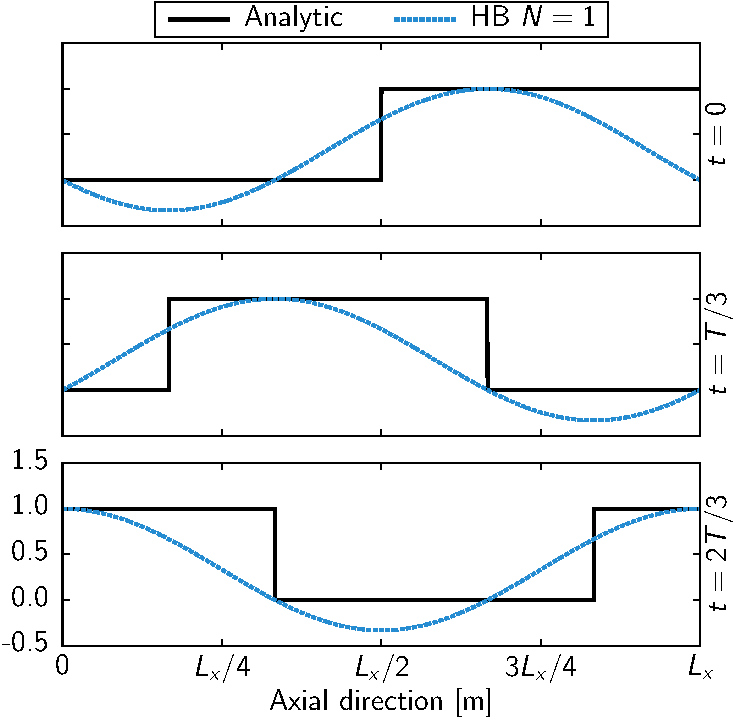
\includegraphics[width=.35\textwidth]{convection_step_N1.pdf}}
  \subfigure[$N=2$]{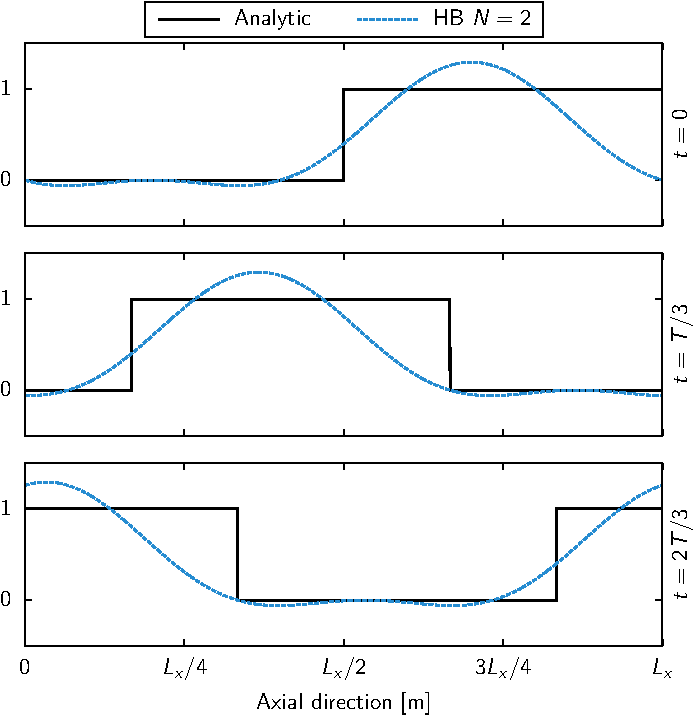
\includegraphics[width=.35\textwidth]{convection_step_N2.pdf}}
  \subfigure[$N=3$]{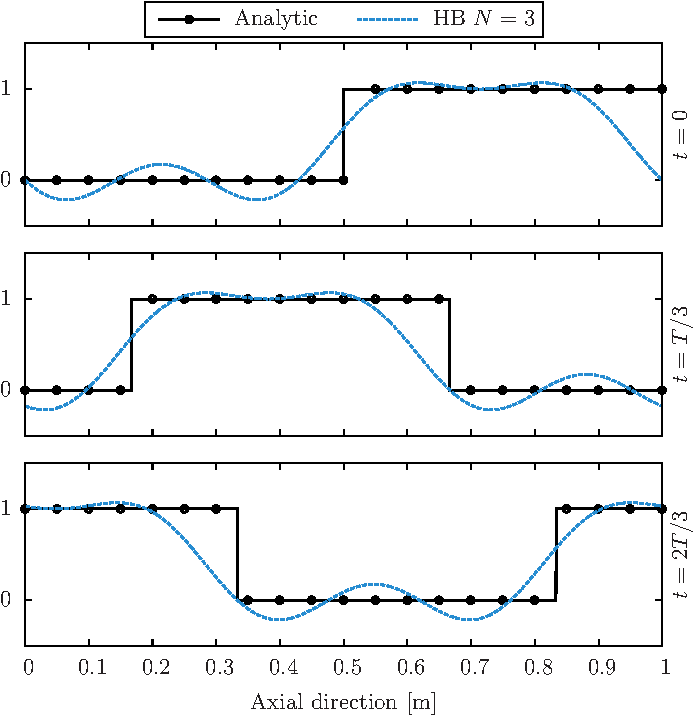
\includegraphics[width=.35\textwidth]{convection_step_N3.pdf}}
  \subfigure[$N=4$]{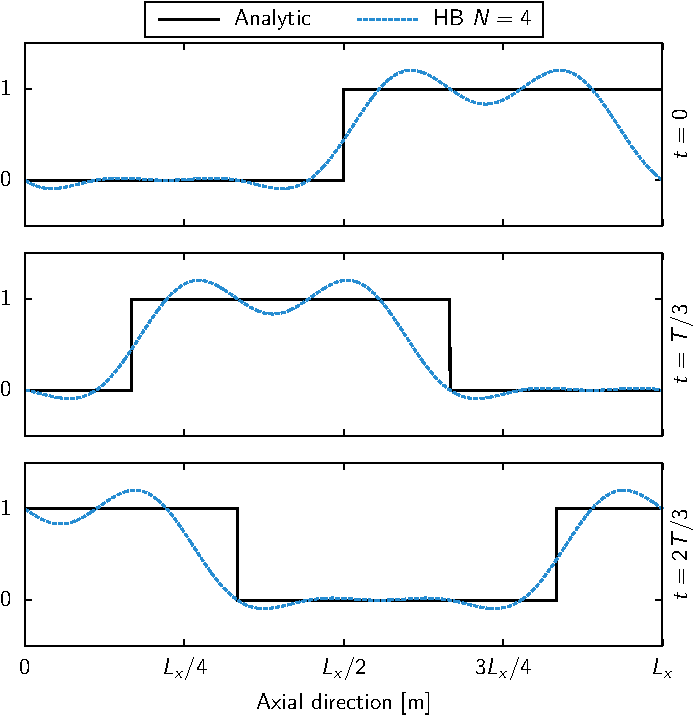
\includegraphics[width=.35\textwidth]{convection_step_N4.pdf}}
  \subfigure[$N=5$]{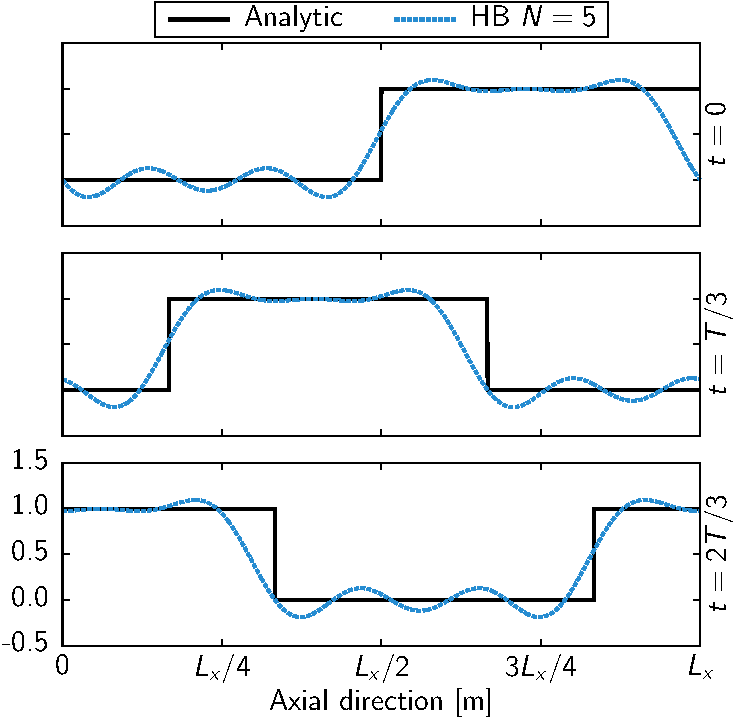
\includegraphics[width=.35\textwidth]{convection_step_N5.pdf}}
  \subfigure[$N=6$]{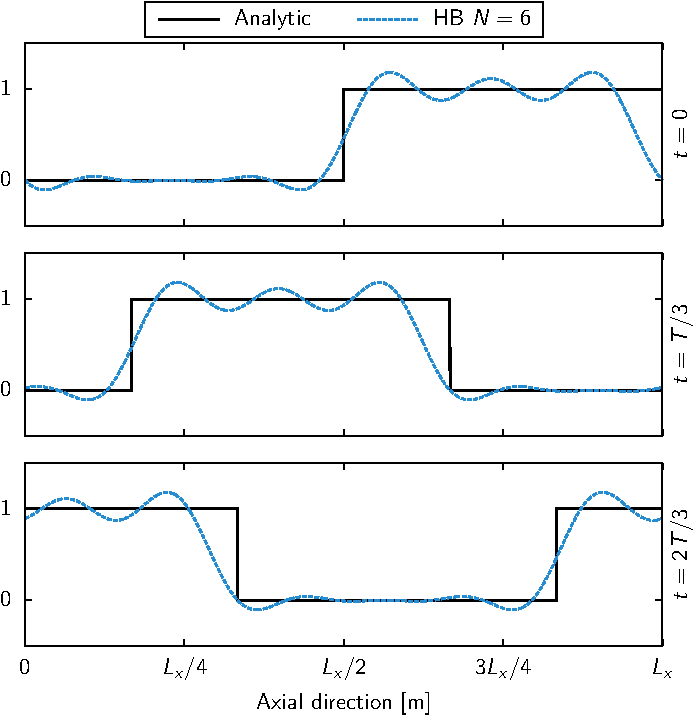
\includegraphics[width=.35\textwidth]{convection_step_N6.pdf}}
  \caption{Linear advection of a rectangular function: 
  numerical solutions at different time instances for different numbers of harmonics.}

  \label{fig:inj_step_results}
\end{figure}

Figure~\ref{fig:inj_step_results} depicts the results of HB computations
using one to six harmonics at different time instances. The convergence rate 
is slow, and for the six-harmonics HB computation the
shape of the rectangular function is still barely captured. 
The well-known \citet{Gibbs1899}
phenomenon is observed, which is a typical drawback 
of Fourier-based methods applied to discontinuous problems, 
see \emph{e.g.} \citet{Canuto2006}.

\begin{figure}[htp]
  \centering
  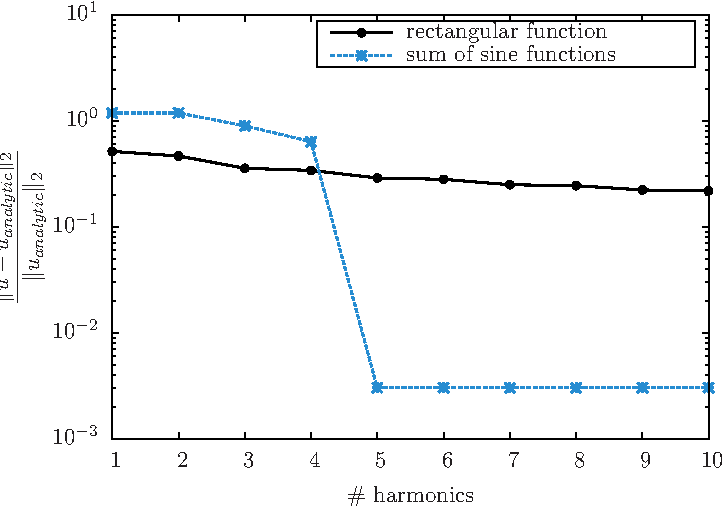
\includegraphics[width=.5\textwidth]{convection_step_error.pdf}
  \caption{Linear advection of a rectangular function: convergence of the HB method error.}
  \label{fig:conv_step}
\end{figure}
As for the previous case, the $\mathcal{L}_2$-norm 
of the error is depicted in Fig.~\ref{fig:conv_step}. 
The convergence of the sum of sine functions, that has been studied in Sec.~\ref{sec:sum_sine},
is added for comparison.
The convergence rate is dramatically different from the previous one: 
the error decreases slowly when more harmonics are introduced, 
but the exact solution is never reached, 
unless an infinite number of harmonics is considered.

The discrete Fourier transform of the results
is computed and compared to the analytical result in Fig.~\ref{fig:dft_step}.
For this case, the spectrum in not finite and cannot be captured accurately
with a finite number of samples.

\begin{figure}[htp]
  \centering
  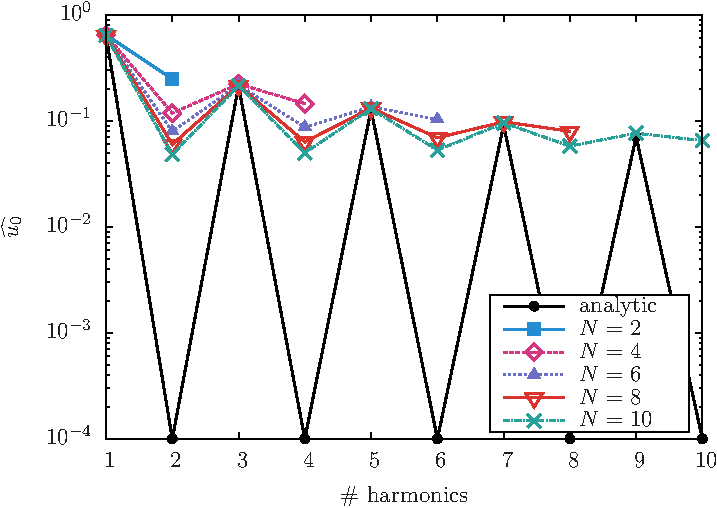
\includegraphics[width=.5\textwidth]{convection_step_dft.pdf}
  \caption{Linear advection of a rectangular function: 
  discrete Fourier transform.}
  \label{fig:dft_step}
\end{figure}